\section{CEGAR}
\subsection{CEGAR and interpolation in general}
\begin{figure}[t]
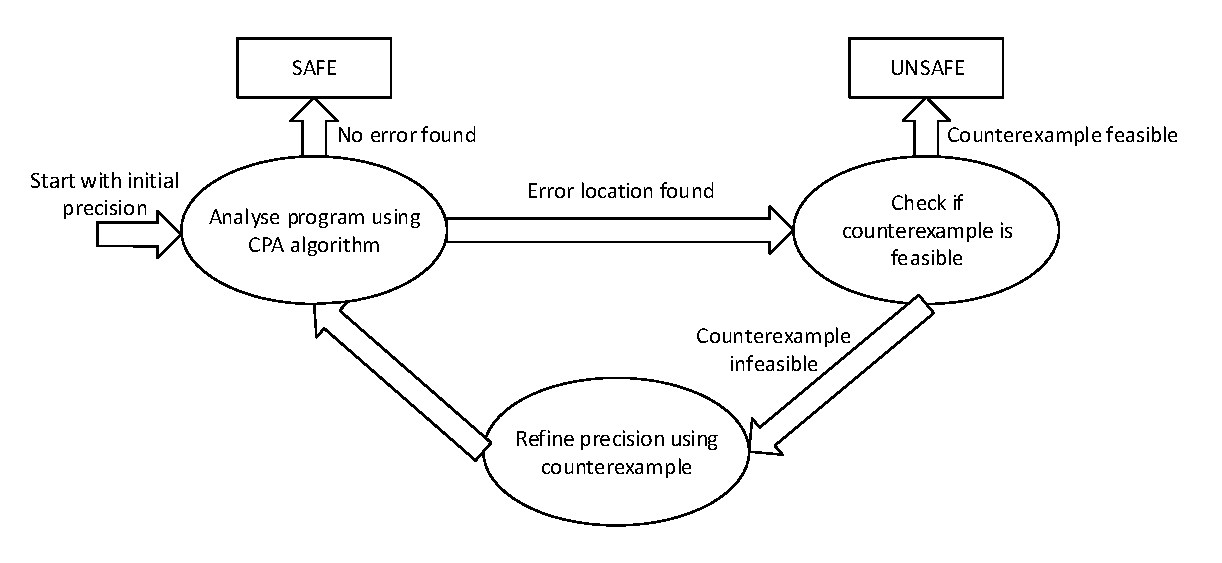
\includegraphics[width=\linewidth]{theoreticalBackground/CegarPrinciple}
\caption{The general idea of CEGAR}
\label{fig:cegarPrinciple}
\end{figure}
Counterexample-guided abstraction refinement (CEGAR) \cite{Clarke2003} is a technique to find an abstraction that contains as few information as possible while retaining the possibility to prove or disprove a program's correctness.
This technique can greatly reduce the number of abstract states in a program's analysis and is considered ''the most general and flexible for handling the state explosion problem,''\cite{Clarke2003}\ the major problem we are facing with our \symbolicExecutionCPA.

The technique starts analysis with a coarse abstraction and refines it based on counterexamples. A counterexample is a witness of a property violation.\cite{Beyer2013}
If no error path is found by the analysis, it terminates and reports that no property violation exists.
If an error path is found, it is checked whether the path is feasible (i.e. a possible program execution) by repeating the analysis with full precision.
If the path is feasible, the analysis terminates and reports the found property violation.
If the error path is infeasible it was only found because the abstraction is too coarse. As a consequence, the abstraction is refined using the error path.
After this, the analysis starts again, using the new abstraction.

Since the problem of finding the coarsest possible refinement of an abstraction based on an error path is NP-hard, \cite{Clarke2003}\ good heuristics have to be used to find good refinements.
Interpolation \cite{Henzinger2004}\ is one such technique originally proposed for model checking.
As such stemming from a boolean context, we use interpolation for refinement of both the \predicateCPA\ and \valueAnalysisCPA.

\subsection{CEGAR and interpolation in the context of configurable software verification}
\label{sec:cegarBasics}

\begin{algorithm}[t]
\caption{$CEGAR(\cpaPlus, e_0, \pi_0)$, adapted from \cite{Beyer2013}}
\label{alg:cegar}
\begin{algorithmic}[1]
\Input a CPA $\cpaPlus = (D, \Pi, \transfer, \cpaMerge, \cpaStop, \cpaPrec)$ with dynamic precision adjustment,
	an initial abstract state $e_0 \in E$ with precision $\pi_0 \in \Pi$,
	with $E$ denoting the set of elements of the semi-lattice of $D$
\Output the verification result \safe\ or \unsafe
\Variables the sets \reachedSet\ and \waitlistSet\ of elements of $E \times \Pi$,
	      an error path $\sigma = \langle (op_1, l_1), ..., (op_n, l_n) \rangle$\\

\State $\reachedSet \assign \{ (e_0, \pi_0) \}$
\State $\waitlistSet \assign \{ e_0, \pi_0 \}$
\State $\pi \assign \pi_0$
\While{true}
	\State $(\reachedSet, \waitlistSet) \assign CPA(\cpaPlus, \reachedSet, \waitlistSet)$
	\If{$\waitlistSet = \varnothing$}
		\Return \safe
	\Else
		\State $\sigma \assign \extractErrorPath{\reachedSet}$ \label{alg:cegar:extraction}
		\If{\isFeasible{$\sigma$}} \Comment error path feasible: report bug \label{alg:cegar:feasibilityCheck}
			\State % empty state for new line after if
			\Return \unsafe 
		\Else \Comment error path infeasible: refine and restart from the beginning
			\State $\pi \assign \pi \cup \refine{\sigma}$
			\State $\reachedSet \assign (e_0, \pi)$
			\State $\waitlistSet \assign (e_0, \pi)$ \label{alg:cegar:end}
		\EndIf
	\EndIf
\EndWhile
\end{algorithmic}
\end{algorithm}

The CEGAR algorithm displayed in Alg.~\ref{alg:cegar} uses a CPA using dynamic precision adjustment $\cpaPlus$,
an initial state $e_0$
and an initial precision $\pi_0$
to compute whether a property violation exists.

First, the $CPA$ algorithm is used to compute a set of reached abstract states ($\reachedSet$) and a subset of this set that contains all reached abstract states that have not been handled yet ($\waitlistSet$).
If $\waitlistSet$ is empty, the $CPA$ algorithm has handled all reachable states without encountering any target state.
If this is the case, no property violation was found and the algorithm can return \safe.
Otherwise, an error path is extracted from the reached set.
If the error path is reported as feasible, a property violation exists or the algorithm is not able to prove that none exists. It returns \unsafe.
If the error path is infeasible, the current precision is too abstract.
It is refined based on the infeasible error path by using $\refineFunc : \Sigma \rightarrow \Pi$ with $\Sigma$ being the set of all error paths, so that it can prove its infeasibility.
After this, the reached set and waitlist are reset to their initial values and the algorithm repeats analysis with the refined precision.
It is important to notice that the return type of $\refineFunc$ has to be equal to the precision type $\Pi$ used in $\cpaPlus$.
Because of this, CPAs are not exchangeable without changing refinement, too, in general.

%%%%%%%%%%%%%%%%%%%%%%%%%%
%%% Refinement in general
%%%%%%%%%%%%%%%%%%%%%%%%%%
For refinement, the priorly mentioned technique of interpolation is used to determine a location-specific precision that is strong enough for the CPA algorithm with precision adjustment to prove that a given error path is infeasible.
A boolean formula $\craigItp$ is a Craig interpolant \cite{Craig1957}\ for two boolean formulas $\prefix$ (called prefix) and $\suffix$ (called suffix), if the following three conditions are fulfilled:
\begin{enumerate}[label=\alph*)]
\item The prefix implies $\craigItp$, that is $\prefix \Rightarrow \craigItp$.
\item $\craigItp$ contradicts the suffix, that means $\craigItp \logicAnd \suffix$ is contradicting.
\item $\craigItp$ only contains variables occurring in \emph{both} prefix and suffix.
\end{enumerate}
It is proven that such an interpolant always exists in the domain of abstract variable assignments \cite{Beyer2013} as well as in the theory of linear arithmetic \cite{Craig1957}.

%\subsubsection{Refinement for the domain of abstract variable assignments}
\label{sec:assignmentRefinement}
Our work is strongly based on the refinement technique for abstract variable assignments.
The strongest-post operator $\strongestPostOp_{op}$ describes the semantics of an operation $op \in Ops$.
It is the analogy to the transfer relation in the domain of CPAs.
It maps a region of concrete states, implied by an abstract variable assignment, to the region of all concrete states that can be reached by executing $op$.
The semantics of a path $\sigma = \langle (l_1, op_1), ..., (l_n, op_n) \rangle$ is defined as the consecutive application of the strongest-post operator to its constraint sequence $\gamma_\sigma = \langle op_1, ..., op_n \rangle$:
$\strongestPostOp_{\gamma_\sigma}(v) = \strongestPostOp_{op_n}(\strongestPostOp_{op_{n-1}} (...\ \strongestPostOp_{op_1}(v) ... ))$.
We use strongest-post operators during interpolation and refinement to evaluate paths.

\subsubsection*{Strongest-post Operator}
The strongest-post operator $\strongestPostOpExplicit_{op}$ is defined in the following way:
%\begin{enumerate}[label=\alph*)]
%\item
For an assignment operation $s \assign exp$, $\strongestPostOpExplicit_{s \assign exp}(v) = v_\restrictedTo{X \setminus \{ s \}} \logicAnd v_{s \assign exp}$ with $v_{s \assign exp} = \{ (s, exp_\using{v}) \}$ and $exp_\using{v}$ denoting the evaluation of $exp$ using the abstract variable assignment $v$, as defined in Section \ref{sec:valueAnalysis}.
%\item
For an assume operation $\assume(p)$, 
	$\strongestPostOpExplicit_{\assume(p)}(v) = v'$ with 
	\[ v'(x) = \begin{dcases}
		\bot & \text{ if } \exists y \in \defRange(v) : v(y) = \bot \text{ or } p_\using{v} \text{ is unsatisfiable}\\
		c & \text{ if $c$ is the only satisfying assignment of $p_\using{v}$ for $x$}\\
		v(x) & \text{ if none of the above and } x \in \defRange(v)
	\end{dcases}\]
	with $p_\using{v}$ as defined in Section \ref{sec:valueAnalysis}.
%\end{enumerate}

\subsubsection*{Interpolation}
%\subsubsection{Interpolation for abstract variable assignments}
\begin{algorithm}[t]
\caption{$\interpolateExplicit(\prefix, \suffix)$, adapted from \cite{Beyer2013}}
\label{alg:interpolateExplicit}
\begin{algorithmic}[1]
\Input two constraint sequences $\prefix$ and $\suffix$, with $\prefix \logicAnd \suffix$ contradicting
\Output a constraint sequence $\Gamma$, which is an interpolant for $\prefix$ and $\suffix$
\Variables an abstract variable assignment $v$

\State $v \assign \strongestPostOpExplicit_\prefix(\varnothing)$
\ForAll{$x \in \defRange(v)$}
	\If{$\strongestPostOpExplicit_\suffix(v_\restrictedTo{\defRange(v) \setminus \{x\}})$ is contradicting}
		\State $v \assign v_\restrictedTo{\defRange(v) \setminus \{x\}}$ \Comment $x$ not relevant, should not occur in interpolant
	\EndIf
\EndFor
\State $\Gamma \assign \langle \rangle$
\ForAll{$x \in \defRange(v)$} \label{alg:interpolateExplicit:itpStart}
	\State $\Gamma \assign \Gamma \logicAnd \langle \assume(x = v(x))\rangle$
\EndFor\\ \label{alg:interpolateExplicit:itpFinish}
\Return $\Gamma$
\end{algorithmic}
\end{algorithm}

The algorithm for interpolation in the domain of abstract variable assignments is shown in Algorithm \ref{alg:interpolateExplicit}.
For a prefix $\prefix$ and a suffix $\prefix$, the abstract variable assignment $v$, that results from applying $\prefix$ to the initial abstract variable assignment $\varnothing$ is computed.
Next, for each variable assignment in $v$ it is checked whether the assignment is necessary to prove that $\suffix$ is contradicting.
If it is not, it can be removed from $v$.
After all variable assignments are checked, $v$ only contains variable assignments that are necessary to prove that $\suffix$ is contradicting.
From these, the interpolant is built (Lines \ref{alg:interpolateExplicit:itpStart} - \ref{alg:interpolateExplicit:itpFinish}).

\subsubsection*{Refinement}
\begin{algorithm}[t]
\caption{$\refineExplicit{\sigma}$, adapted from \cite{Beyer2015}}
\label{alg:refinementExplicit}
\begin{algorithmic}[1]
\Input infeasible error path $\sigma = \langle (op_1, l_1), ..., (op_n, l_n) \rangle$
\Output precision $\pi$
\Variables interpolating constraint sequence $\Gamma$
\State $\Gamma \assign \langle \rangle$
\State $\pi(l) \assign \varnothing$ for all program locations $l$
\For{$i \assign 1$ to $n - 1$}\label{alg:refinementExplicit:loopStart}
	\State $\suffix \assign \langle op_{i+1}, ..., op_n \rangle$
	\State $\Gamma \assign \interpolateExplicit(\Gamma \logicAnd \langle op_i \rangle, \suffix)$ \Comment inductive interpolation \label{alg:refinementExplicit:interpolation}
	\State $\pi(l_i) \assign \extractPrecision{\Gamma}$
\EndFor\\
\Return $\pi$
\end{algorithmic}
\end{algorithm}

The interpolants produced are used in the refinement of the precision (Alg. \ref{alg:refinementExplicit}).
We use a location-specific precision $\pi : L \rightarrow 2^X$ that returns for a program location $l \in L$ all program variables of $X$ which are relevant for the analysis at this location. 
The algorithm starts with an initial, empty interpolant $\Gamma$ and empty precision $\pi$ with $\pi(l) = \varnothing$ for all $l \in L$.
For each location $(l_i, op_i)$ on the error path, the suffix $\suffix$ of this location are set and the interpolant is computed inductively from the existing interpolant in conjunction with the current operation $op_i$ and the suffix (Line \ref{alg:refinementExplicit:interpolation}).
A precision for the current program location is then extracted from the interpolant.
One straightforward way to do this is by using all program variables with a valid assignment in the  abstract variable assignment resulting from the application of the strongest-post operator to our interpolant:
\[\extractPrecision{\Gamma} = \{ x |\ (x, z) \in \strongestPostOpExplicit_\Gamma (\varnothing ) \text{ and } z \neq \bot_\valueset \}.\]
It is not only sufficient, but also required to use $\Gamma \logicAnd \langle op_i \rangle$ instead of the full prefix $\prefix = \langle op_1, ..., op_1 \rangle$ for interpolation. The full prefix cannot be used as it has to be assured that the precision resulting from these consecutive interpolations proves the error path infeasible. All information necessary for proving the infeasibility of the remaining error path is present in the current interpolant and operation.

This refinement procedure can be used in CEGAR (Alg. \ref{alg:cegar}) in combination with a CPA with precision adjustment that expects these precision types, like the \valueAnalysisCPA\ in combination with refinement for abstract variable assignments.

\subsubsection*{Lazy Abstraction}
Resetting the reached set and waitlist to their initial values after every refinement results in the CPA algorithm starting at the first state, always.
Most of the time, this is not actually necessary though, because precision only changed for a few program locations.
Because of this, lazy abstraction \cite{Henzinger2002} resumes analysis not at the beginning of the CFA, but at the first location that has to be revisited with its new precision so that the current error path is computed as infeasible.
This location is the one before the first pair $(op_i, l_i)$ whose corresponding interpolant is not the empty constraint sequence (i.e. the location before the first location with a new precision).
We realize lazy abstraction by not resetting the waitlist and reached set in the CEGAR algorithm after each refinement procedure to $(e_0, \pi_0)$.
Instead, only abstract states for locations whose precision has changed and all their children are removed from the reached set and added to the waitlist.
This way redundant computations without any finer precision are avoided.

\subsubsection*{Using Path Prefix Selection}
When computing the interpolant for a prefix and a suffix, the resulting interpolant is random if more than one possible interpolant exist. But some interpolants are better suited for creating a precision reaching a fast termination of analysis than others.
The enhanced refinement procedure proposed by \cite{Beyer2015} allows to guide the interpolation process based on arbitrary criteria.
A sliced path prefix is a path in an error path $\sigma$ resulting from omitting pairs of operations and locations from the end and replacing assume operations by no-op operations. If a sliced prefix of $\sigma$ is infeasible, $\sigma$ is infeasible.\cite{Beyer2015}

\begin{algorithm}[t]
\caption{$\refinePlus{\sigma}$, taken from \cite{Beyer2015}}
\label{alg:refinementPlus}
\begin{algorithmic}
\Input an infeasible error path $\sigma = \langle (op_1, l_1), ..., (op_n, l_n) \rangle$
\Output a precision $\pi \in L \rightarrow 2^\Pi$
\Variables a set $\Sigma$ of infeasible sliced prefixes of $\sigma$,
           a mapping $\tau$ from infeasible sliced prefixes and program locations to precisions, and
           a sliced path prefix $\phi_{selected}$
\State $\Sigma \assign \extractSlicedPrefixes{\sigma}$
\Comment compute precisions for each infeasible sliced prefix
\ForAll{$\phi_j \in \Sigma$}
  \State $\tau(\phi_j) \assign \refineExplicit{\phi_j}$ \Comment Alg.~\ref{alg:refinementExplicit}
\EndFor
\Comment select suitable sliced prefix based on the prefix and its precision
\State $\phi_{selected} \assign \selectSlicedPrefix(\tau)$
\Comment return precision for CEGAR based on selected sliced prefix
\Return $\tau(\phi_{selected})$
\end{algorithmic}
\end{algorithm}

Algorithm~\ref{alg:refinementPlus} shows the enhanced refinement procedure.
For a given error path $\sigma$, all infeasible sliced prefixes are extracted using $\extractSlicedPrefixesFunc$.
For each such sliced prefix, refinement as described above is performed to derive a precision sufficient to prove $\sigma$ infeasible.
After this, one such precision is selected based on the prefix and its precision and returned to be used with CEGAR.

\begin{algorithm}[t]
\caption{$\extractSlicedPrefixes{\sigma}$, taken from \cite{Beyer2015}}
\label{alg:extractPrefixes}
\begin{algorithmic}
\Input infeasible path $\sigma = \langle (op_1, l_1), ..., (op_n, l_n) \rangle$
\Output non-empty set $\Sigma = \{\sigma_1, ..., \sigma_m \}$ of infeasible sliced prefixes of $\sigma$
\Variables a path $\sigma_f$ that is always feasible
\State $\Sigma \assign \varnothing$
\State $\sigma_f \assign \langle \rangle$
\ForAll{$(op, l) \in \sigma$}
  \If{$\strongestPostOp_{\sigma_f \logicAnd (op, l)}(\varnothing) = \bot$}
    \Comment $\sigma_f \logicAnd (op, l)$ is an infeasible sliced prefix
    \State $\Sigma \assign \Sigma \cup \{ \sigma_f \logicAnd (op, l) \}$
    \State $\sigma_f \assign \sigma_f \logicAnd ([true], l)$ \Comment append no-op to be able to continue
  \Else
    \State $\sigma_f \assign \sigma_f \logicAnd (op, l)$ \Comment append original pair
  \EndIf
\EndFor
\Return $\Sigma$
\end{algorithmic}
\end{algorithm}

The algorithm for extracting all infeasible prefixes is shown in Alg.~\ref{alg:extractPrefixes}.
For each operation $(op, l)$ on a given infeasible path $\sigma$, it is checked whether it is contradicting with the already computed path $\sigma_f$, which is always feasible.
If it is contradicting, the path $\sigma_f \logicAnd (op, l)$ is added to the set of infeasible sliced prefixes
and the operation doing nothing (no-op), $[true], l)$ is appended to $\sigma_f$ so that it stays feasible and new infeasible prefixes can be found using it.
If it is not contradicting, $\sigma_f$ is just extended by $(op, l)$.
After this, the next operand-location pair on the path is examined.

This enhanced refinement procedure allows to enhance CEGAR by selecting precisions best fit for analysis.

\subsubsection*{Refinement for the domain of linear arithmetic}
Refinement in the domain of linear arithmetic, as used for the \predicateCPA, uses a standard approach to refinement based on lazy abstraction and Craig interpolation.
The task of interpolation is delegated to an off-the-shelf SMT solver.

%\subsubsection{\ValueAnalysisCPA\ with precision adjustment}
%The \valueAnalysisCPA\ with dynamic precision adjustment \cite{Beyer2013} \[\valCPAPlus = (D_\valCPA, \Pi_\valCPAPlus, \transfer_\valCPAPlus, \cpaMerge^{sep}, \cpaStop^{sep}, %\cpaPrec_\valCPAPlus)\] is a CPA that can be, and is, used with the refinement for abstract variable assignments as described above.
%It consists of:
%\begin{enumerate}[leftmargin=*, label=\arabic*.]
%\item The abstract domain $D_\valCPA$ as defined in Section \ref{sec:valueAnalysis}.
%\item The set of precisions $\Pi_\valCPAPlus = L \rightarrow 2^X$. A precision $\pi \in \Pi_\valCPAPlus$ specifies a subset of program variables of $X$ that are tracked.
%\item The transfer relation $\transfer_\valCPAPlus$ contains the transfer $v \transfer_\valCPAPlus (v', \pi)$ if $v \transfer_\valCPA v'$.
%\item The merge operator $\cpaMerge^{sep}$ that performs no merging.
%\item The termination check $\cpaStop^{sep}$ that checks every state individually.
%\item The precision adjustment $\cpaPrec_\valCPAPlus$. Given an abstract state $v$ and a precision $\pi$, all abstract assignments of variables that do not occur in $\pi$ are removed from %$v$. This is done by restricting the partial function: $\cpaPrec_\valCPAPlus(v, \pi) = (v_\restrictedTo{\pi}, \pi)$. The given precision is returned as it is.
%\end{enumerate}

In this chapter, we gave an overview of all theoretical concepts that are necessary to describe our own work. We introduced the concept of configurable software verification and configurable program analyses (CPAs), a very versatile approach to automated software verification. We introduced different CPAs we use in this work and CEGAR with precision refinement for both linear arithmetic and abstract variable assignments, which we will use when applying CEGAR to the \symbolicExecutionCPA.
